\section{Results}

% \begin{frame}
% How do we make these happen?
% \begin{align*}
% \sum_F \flat_F &\leftrightsquigarrow \int_M K\,dA  \\
% \sum_F I^X_F &\leftrightsquigarrow  \sum_{i=1}^{n} \mathsf{index}_{x_i} \\
% ? &\leftrightsquigarrow \frac{1}{2\pi}\int_M K\,dA - \sum_{i=1}^{n} \mathsf{index}_{x_i} = 0 
% \end{align*}
% \end{frame}

\begin{frame}
\begin{itemize}
\item On a single face we have \( I^X_F=\loopy(\flat_F(X_1)\cdot X_F) \).
\item Map \( \flat_F(X_1) \) and \( X_F \) to angles in \( T_m=T_m \).
\item Sum over faces can be performed in \( T_m=T_m \).
\item Assume that each edge is traversed twice, once in each direction.
\item Prove that the total angle \( \sum_F X_F=0 \).
\item Leaving us \( I_\mathrm{tot}=\loopy(\flat_{\mathrm{tot}}) \).
\end{itemize}
\end{frame}

\begin{frame}{Classical proof}
\begin{columns}
\column{0.5\textwidth}
\vspace{12pt}
\begin{figure}
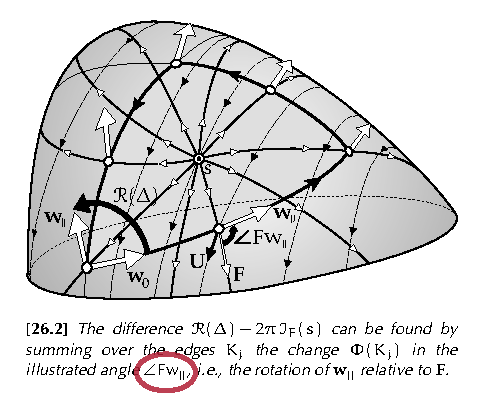
\includegraphics[width=0.9\textwidth]{figs/needham_triangle_circ.pdf}
\caption{{Needham,~T. (2021) Visual Differential Geometry and Forms.}}
\end{figure}
\column{0.5\textwidth}
\vspace{-12pt}
\begin{itemize}
\item The classical proof is discrete-flavored.
\item ``\( \angle Fw_{||} \)'' looked a lot like a pathover.
\item Hopf's \( \Phi \) is defined on edges, not loops. We imitated that too.
\end{itemize}
\end{columns}
\end{frame}
